\paragraph{} Este apêndice contêm a descrição de algumas arquiteturas de rede neural usadas neste trabalho, além de descrever os hiperparâmetros de cada rede.

\paragraph{} Alguns hiperparâmetros são comuns a todos os modelos, são eles:
\begin{itemize}
	\item \textbf{Comprimento da Janela de Entrada} : Número de instantes de tempo passados usados como entrada para o modelo.
	\item \textbf{Comprimento da Janela de Saída}   : Número de passos à frente que o modelo prevê.
	\item \textbf{Comprimento do Lote} : especifica o número de amostras processadas simultaneamente durante o treinamento, o que afeta tanto a eficiência computacional quanto a qualidade da convergência.
	\item \textbf{Número de Épocas} : Número de vezes que o modelo passa por todo o conjunto de treinamento.
	\item \textbf{Taxa de Aprendizado}: Define a rapidez com que o modelo ajusta os pesos das conexões durante o treinamento.
	\item \textbf{Otimizador} : Algoritmo que ajusta os pesos das conexões durante o treinamento.
	\item \textbf{Função de Perda} : Função que calcula a diferença entre a previsão e o valor real.
\end{itemize}

\section{\acf{NARX}}
\paragraph{} O modelo \ac{NARX} é uma classe de modelos não lineares, onde a saída y(n+1) é uma função dos valores de entrada e dos valores atrasados da saída, conforme mostra a Equação \ref{eq:narx} \cite{haykin1998neural}.

\begin{equation}
	y(n+1) = f^l(x(n), x(n-1), \hdots, x(n-p), y(n-q), \hdots, y(n))
	\label{eq:narx}
\end{equation}
\paragraph{} Sendo \(f^l\) a função não-linear de grau \(l\) do modelo, \(y\) os valores de saída, \(x\) os valores de entrada do modelo, \(n\) o instante de tempo atual, \(p\) o número de atrasos aprensentados ao modelo na entrada, \(q\) o número de atrasos recuperados da saída para a entrada e \(o\) o horizonte de previsão. O diagrama de blocos do modelo \ac{NARX} é mostrado na Figura \ref{fig:narx_diagram}.

\begin{figure}
	\begin{center}
		\begin{center}
			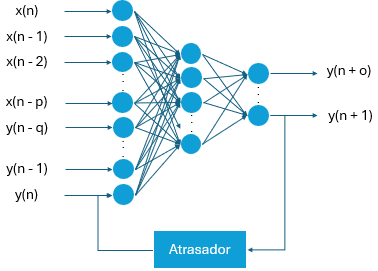
\includegraphics[width=0.8\textwidth]{figuras/narx_diagram.png}
			\caption{Diagrama da \acs{NARX}}
			\label{fig:narx_diagram}
			\text{Fonte: Elaborado pelo autor, baseado em \cite{haykin1998neural}}
		\end{center}

	\end{center}
\end{figure}

\paragraph{} Os principais hiperparâmetros que ajustam o treinamento do modelo são:
\begin{itemize}
	\item \textbf{Tamanho da Camada Escondida}      : Número de neurônios nas camadas escondidas, influenciando a capacidade de abstração do modelo.
	\item \textbf{Número de Atrasos na Entrada}		: Número de atrasos apresentados ao modelo na entrada, influenciando a capacidade de capturar dependências temporais.
\end{itemize}

\section{\acf{DA-RNN}}

\paragraph{} O modelo \ac{DA-RNN} representa uma abordagem alternativa, baseada em \ac{RNN} para a previsão de séries temporais. Este modelo é projetado para lidar com dados sequenciais, utilizando um mecanismo de atenção em duas etapas, o que melhora a precisão das previsões ao capturar dependências de longo prazo \cite{zheng2017forecasting}. O diagrama é mostrado na Figura \ref{fig:darnn_diagram}.

\begin{figure}
	\begin{center}
		\begin{center}
			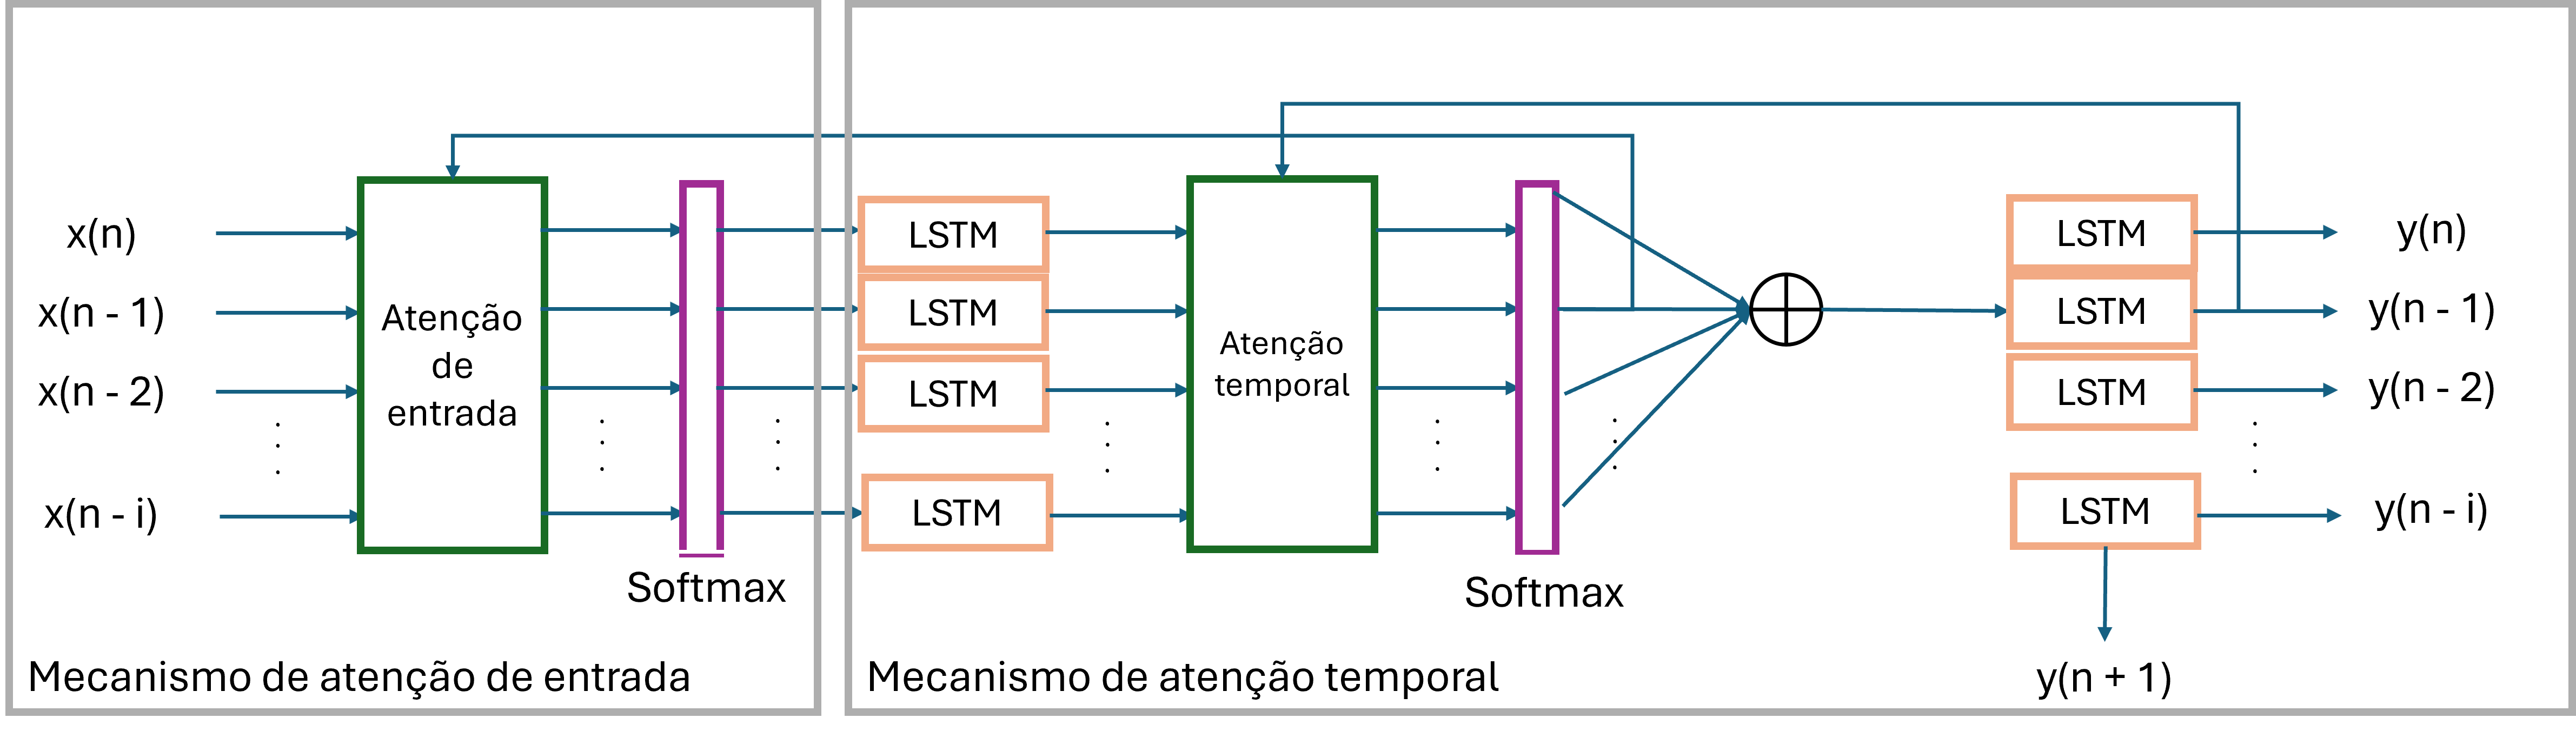
\includegraphics[width=1\textwidth]{figuras/darnn_diagram.png}
			\caption{Diagrama da \acs{DA-RNN}}
			\label{fig:darnn_diagram}
			\text{Fonte: Elaborado pelo autor, baseado em \cite{zheng2017forecasting}}
		\end{center}

	\end{center}
\end{figure}

\paragraph{} Sendo \(x\) o vetor de entradas, \(n\) o instante atual, \(y\) o vetor de saídas e \(i\) o tamanho da janela de entrada.

\paragraph{} Os principais hiperparâmetros que ajustam o treinamento do modelo são:
\begin{itemize}
	\item \textbf{Tamanho da Camada Escondida}      : Número de neurônios nas camadas escondidas, influenciando a capacidade de abstração do modelo.
	\item \textbf{Número de Cabeças de Atenção}		: Número de cabeças no mecanismo de atenção, permitindo ao modelo focar em diferentes partes da sequência de entrada.
	\item \textbf{Taxa de Abandono (do inglês \textit{dropout})}                 : Fração de neurônios que são desativados durante o treinamento, evitando o sobreajuste.
\end{itemize}

\section{\acf{MLP}}

\paragraph{} A \ac{MLP} é uma rede neural feedforward composta por múltiplas camadas de neurônios. Cada neurônio aplica uma função de ativação a uma combinação linear das entradas, permitindo modelar relações não lineares, como mostrado na Equação \ref{eq:mlp}. A estrutura básica envolve uma camada de entrada, uma ou mais camadas ocultas e uma camada de saída. O aprendizado é realizado por meio do algoritmo de retropropagação, que ajusta os pesos das conexões para minimizar a diferença entre a previsão e a saída desejada \cite{haykin1998neural}. O diagrama é mostrado na Figura \ref{fig:mlp_diagram}.
\begin{equation}
	y = W_{2} \sigma(W_{1} x + b_{1}) + b_{2}
	\label{eq:mlp}
\end{equation}
\paragraph{} Sendo \( x \) o vetor de entrada, \( W_1 \) e \( W_2 \) as matrizes de pesos da camada de entrada para a camada oculta e da camada oculta para a camada de saída, respectivamente, \( b_1 \) e \( b_2 \) os vetores de bias e \( \sigma \) uma função de ativação não linear.

\begin{figure}
	\begin{center}
		\begin{center}
			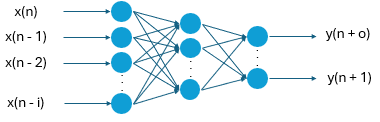
\includegraphics[width=0.8\textwidth]{figuras/mlp_diagram.png}
			\caption{Diagrama da \acs{MLP}}
			\label{fig:mlp_diagram}
			\text{Fonte: Elaborado pelo autor, baseado em \cite{haykin1998neural}}
		\end{center}

	\end{center}
\end{figure}

\paragraph{} Os principais hiperparâmetros que ajustam o treinamento do modelo são:
\begin{itemize}
	\item \textbf{Tamanho da Camada Escondida}      : Número de neurônios nas camadas escondidas, influenciando a capacidade de abstração do modelo.
\end{itemize}

\section{\acf{IMP}}

\paragraph{} O modelo \ac{IMP} consiste em uma combinação convexa entre duas decomposições morfológicas, por erosões e dilatações. Como mostrado em Araújo, 2012 \cite{araujo_morphological_2012} na Figura \ref{fig:imp_diagram}.

\begin{figure}
	\begin{center}
		\begin{center}
			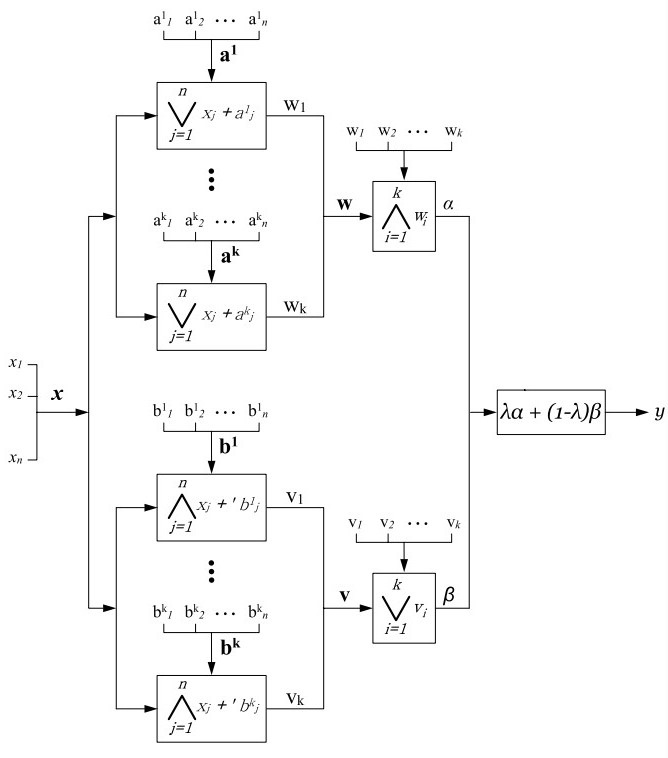
\includegraphics[width=0.8\textwidth]{figuras/imp_diagram.jpg}
			\caption{Diagrama da \acs{IMP}}
			\label{fig:imp_diagram}
			\text{Fonte: Araújo, 2012 \cite{araujo_morphological_2012}}
		\end{center}

	\end{center}
\end{figure}
\paragraph{} Sendo \(n\) o tamanho da janela de entrada, \(\alpha\) a decomposição de operadores morfológicos crescentes por dilatações, \(\beta\) a decomposição de operadores morfológicos crescentes por erosões, \(v\) e \(w\) são os vetores que definem seus respectivos operadores morfológicos.

\paragraph{} Os principais hiperparâmetros que ajustam o treinamento do modelo são os comuns a todos os modelos.

\section{\acf{IDLN}}

\paragraph{} O modelo \ac{IDLN} consiste em uma combinação de operadores morfológicos de dilatação, erosão, anti-dilatação e anti-erosão. Conforme mostrado em Araújo, 2016 \cite{Araujo16} na Figura \ref{fig:idln_diagram}.

\begin{figure}
	\begin{center}
		\begin{center}
			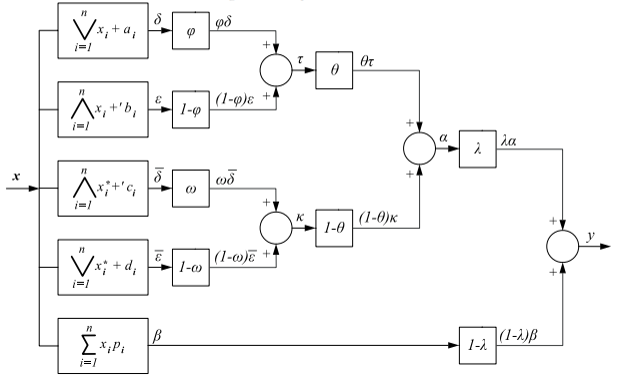
\includegraphics[width=0.8\textwidth]{figuras/idln_diagram.png}
			\caption{Diagrama da \acs{IDLN}}
			\label{fig:idln_diagram}
			\text{Fonte: Araújo, 2016 \cite{Araujo16}}
		\end{center}

	\end{center}
\end{figure}

\paragraph{} Os principais hiperparâmetros que ajustam o treinamento do modelo são os comuns a todos os modelos.

\section{\acf{N-Linear}}

\paragraph{} O modelo \ac{N-Linear} possui uma arquitetura simples, semelhante ao \ac{MLP}, com a camada de entrada sendo substituída por uma etapa de normalização. Onde cada entrada é subtraída do último valor da sequencia, de modo a evitar outliers \cite{DLinear22}. O diagrama é mostrado na Figura \ref{fig:nlinear_diagram}.

\begin{figure}
	\begin{center}
		\begin{center}
			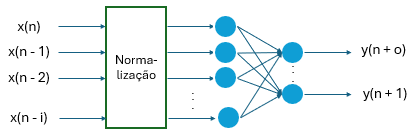
\includegraphics[width=0.8\textwidth]{figuras/nlinear_diagram.png}
			\caption{Diagrama da \acs{N-Linear}}
			\label{fig:nlinear_diagram}
			\text{Fonte: Elaborado pelo autor, baseado em \cite{DLinear22}}
		\end{center}

	\end{center}
\end{figure}

\paragraph{} Os principais hiperparâmetros que ajustam o treinamento do modelo são os comuns a todos os modelos.

\section{\acf{NHiTS}}

\paragraph{} O modelo NHiTS compõe a classe dos modelos de aprendizado profundo. Sua arquitetura é em pilhas e blocos, e o modelo é composto por uma série de \(P\) pilhas, cada pilha é composta por uma série de \(B\) blocos residuais que tem por objetivo zerar os resíduos e cada bloco residual é composto por alguns modelos \ac{MLP} com não linearidades aplicadas pela \ac{ReLU} \cite{NHiTS22}.
\paragraph{} O funcionamento do modelo consiste em dividir o sinal multi-taxa em bandas distintas, para que cada pilha seja especializada em uma banda. Cada pilha possuí blocos residuais, onde o sinal é filtrado por um max pool e passa por 3 fluxos de rede \ac{MLP}, seguido de transformações não lineares e não lineares, para fornecer valores de previsão e retroprojeção. No final a previsão resultante é a soma da previsão de cada pilha com o valor residual da última pilha. O diagrama é mostrado na Figura \ref{fig:nhits_diagram}.

\begin{figure}
	\begin{center}
		\begin{center}
			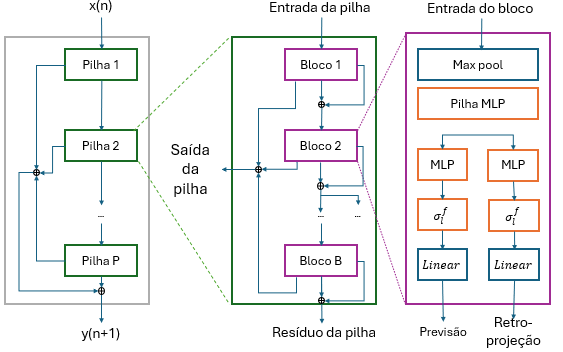
\includegraphics[width=0.8\textwidth]{figuras/nhits_diagram.png}
			\caption{Diagrama da \acs{NHiTS}}
			\label{fig:nhits_diagram}
			\text{Fonte: Elaborado pelo autor, baseado em \cite{NHiTS22}}
		\end{center}

	\end{center}
\end{figure}

\paragraph{} Os principais hiperparâmetros que ajustam o treinamento do modelo são:
\begin{itemize}
	\item \textbf{Número de Pilhas} : Número de pilhas independentes de blocos (\textit{NHiTSBlock}) que compõem a arquitetura. Cada pilha pode aprender diferentes padrões temporais.
	\item \textbf{Número de Blocos} : Número de blocos em cada pilha. Mais blocos permitem que o modelo capture padrões mais complexos ao passar pela rede várias vezes.
	\item \textbf{Número de Camadas} : Número de camadas dentro de cada bloco. Um maior número de camadas adiciona mais profundidade ao modelo, potencialmente melhorando sua capacidade de abstração.
	\item \textbf{Tamanho da Camada} : Número de neurônios por camada dentro de cada bloco. Camadas maiores aumentam a capacidade de aprendizado do modelo.
\end{itemize}